\section{Background: What a Long Session Costs}
\label{sec:background}

\subsection{The replay}

Our workload is a replay of 19 coding-agent sessions (602 rounds) reconstructed from real
Claude and Codex transcripts released with a public coding-agent characterization study
\cite{zhu2026tracelab}. We keep every session with at least 20 rounds and sample by a hash
of the session identifier, which yields the 19 longest sessions rather than a
hand-picked subset; the trace and the script that rebuilds it are in the artifact. Each
round carries the prefix it can reuse, the new tokens it appends, the number of tokens the
model is asked to emit, an inter-round tool wait, and an arrival time. All sessions arrive
at $t=0$: we model the batch-of-agents case (a nightly evaluation, a benchmark sweep, a
fleet of assistants started together), which is the case that stresses admission hardest
and the case an offline batch server is actually configured for.

\begin{figure}[t]
\centering
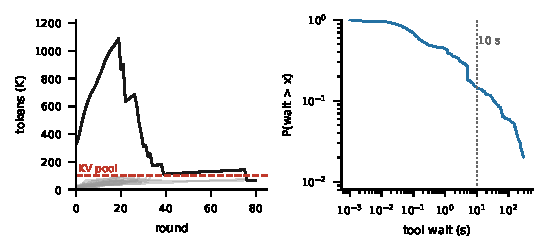
\includegraphics[width=\columnwidth]{figs/fig_workload.pdf}
\caption{Left: the working set if every session alive at that round were resident (black),
against the engine's KV pool (dashed). The aggregate peaks above one million tokens---ten
times the pool---while no single session's context ever exceeds the pool on its own.
Summing every session's terminal context gives 1.31M tokens, $12.9\times$ the pool. Right:
the tool wait between rounds, as a complementary CDF. The distribution is bimodal: half of
the gaps are under 0.2\,s, and the 13.1\% above ten seconds carry 93.4\% of the parked
time.}
\label{fig:workload}
\end{figure}

\subsection{Four numbers that decide the design}

Table~\ref{tab:workload} collects the characterisation and Fig.~\ref{fig:workload}
shows its two shapes; every entry is regenerated from the trace by
\texttt{gen\_trace\_facts.py}. Four of them drive everything that follows.

\paragraph{The working set is an order of magnitude larger than the pool}
The terminal footprint of all 19 sessions is 1.31M tokens. The engine's KV pool on a
24\,GB card with a 96K context and a 7B model is 101.5K tokens. The ratio is
$12.9\times$, and a mean session (69K tokens) already needs two thirds of the pool: the
pool holds 1.47 sessions. There is no scheduling policy that makes 19 sessions resident;
the question is only which subset is resident at each instant.

\paragraph{Almost all of the work is re-reading}
A round appends a median of 990 tokens to a median 44.9K-token prefix. Aggregated over the
trace, the prefix is $13.0\times$ the appended content, and the prefill work of a system
with no reuse would be $14.0\times$ that of a system that never re-reads a prefix. This
gap is the prize: the engine spends its time on prefill of content it has already seen.

\paragraph{Reuse is worth a lot, and it is perishable}
Because a session's context only grows, the prefix of round $i$ is a prefix of round
$i+1$: a single retained copy serves every later round. But retention competes with
admission---every token held for a parked session is a token an active session cannot
use---so reuse and capacity are two views of the same decision, not two separate
optimisations.

\paragraph{Idle time is bimodal, so ``park'' is not one thing}
The median gap between rounds is 181\,ms; the mean is 15.9\,s; the 90th percentile is
28.1\,s and the maximum is the trace's 300\,s timeout. The 13.1\% of gaps above ten
seconds carry 93.4\% of all parked time: across the trace the sessions sit idle for 2.65
hours in total, and 2.47 of those hours are in long gaps. A gap of 181\,ms is shorter than
the cost of moving a 44.9K-token prefix anywhere, while a gap of 28\,s is longer than the
prefill that would rebuild it. Any single policy---always keep, always evict---is wrong
for at least half of the gaps.

\begin{table}[t]
\caption{Workload characterisation of the 19-session, 602-round replay. Context is
measured at the start of a round; the working set sums the terminal context of each
session. All values are recomputed from the trace by \texttt{gen\_trace\_facts.py}.}
\label{tab:workload}
\centering
\small
\begin{tabular}{@{}lr@{}}
\toprule
Quantity & Value \\
\midrule
sessions / rounds & 19 / 602 \\
rounds per session (median / max) & 28 / 81 \\
context per round (median / mean) & 48.5K / 48.2K \\
context per round (p90 / max) & 71.1K / 92.8K \\
terminal working set & 1.31M tokens \\
KV pool (device tier) & 101.5K tokens \\
working set / pool & $12.9\times$ \\
mean session footprint & 69.0K tokens \\
pool in mean sessions & 1.47 \\
appended tokens per round (median) & 990 \\
reusable prefix per round (median) & 44.9K \\
prefix / append, per round (median) & $45.4\times$ \\
prefix / append, whole trace & $13.0\times$ \\
recompute / append bound & $14.0\times$ \\
tool wait p50 / mean & 181\,ms / 15.9\,s \\
tool wait p90 / max & 28.1\,s / 300\,s \\
gaps $>10$\,s (share of gaps / of time) & 13.1\% / 93.4\% \\
\bottomrule
\end{tabular}
\end{table}

\subsection{What a round does to the engine}

A round is a prefill of the full context followed by a short decode: 48.5K tokens in,
about 150 tokens out. On the 24\,GB card the prefill of a cold 44.9K-token prefix takes
about 100\,s (median 103\,s over the 131 cold rounds of one run) and the decode is a fraction of a second; when the
prefix is resident, the same round costs a few milliseconds of copy and a prefill of the
990 new tokens. The engine therefore has two very different operating points, and the
whole question of this paper is how often it can be in the second one.

\subsection{The engine and its memory hierarchy}

We use SGLang \cite{zheng2024sglang} with paged KV \cite{kwon2023pagedattention} and its
hierarchical cache, which extends the device pool with a host pool at a configurable ratio
(we use $2\times$, i.e.\ 203K tokens in host memory). The hierarchy is the substrate that
makes suspension meaningful: the host tier is where a suspended session can wait without
occupying the card, and the PCIe link is the price of putting it back. The engine itself
does not have a notion of a session, so it cannot tell a cache miss caused by a new
session from one caused by an evicted session that is about to return. Supplying that
notion is the job of the design in \S\ref{sec:design}.
